\section{Analysis And visualisation}

Analysis and visualisation are an important aspect in conveying information. In this project, we analysed the data that was processed using the Spark framework. It is very important that we use a big data framework for big data projects. One of the main reason, is that since some data that were collected are bigger than the capacity of the RAM itself, the only way to work on it is to use a clustered system. Spark is one of such framework that take advantage of Hadoop Distributed File System.

There are various reason why visualizing data is important. Visualisation is an important method of conveying information and it lets the viewer have a more holistic and detailed view of the data. It is not uncommon to find deep and new insight of the data through visualisation. It is one of the main method to relay information to all stakeholders, in order to perform a Data-Driven Decision Making (DDDM).

Here we have done plenty visualisation, in term of presenting informative graphics towards the reader. We have done TextCloud visualisation and also scatter plot visualisation for the semantic analysis. The data that was procured from the previous steps were then accessed and prepared for the various visualisations using Pandas framework.

\subsection{Word Analysis and Visualisation}

TextCloud is a very versatile method of presenting information. The group of words are easily read and the main idea of the group of words are relatively comprehensible without deeper analysis. The ability to obtain the big picture efficiently when presenting information to a massive audience is crucial.

The two American political party, The Republican Party and The Democrat Party are two parties that are relatively known for polarized judgement on various topics. In this project, we try to check the most used words by the two parties in Twitter and then see what are the general big ideas that the two parties are most connected to.


\begin{figure}

\centering
  \centering
  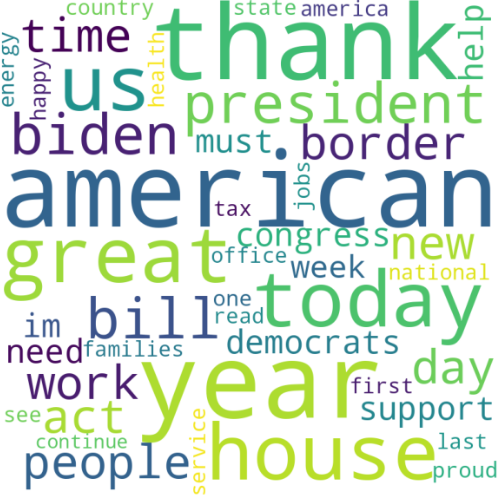
\includegraphics[width=0.7\linewidth]{images/Kapitel3/Republican_word_cloud.png}
%  \caption{Republican Top 50 most used words}
%  \label{fig:sub1}
	\caption{\label{fig:sub1}Republican Top 50 most used words}{}
\end{figure}


\begin{figure}
  \centering
  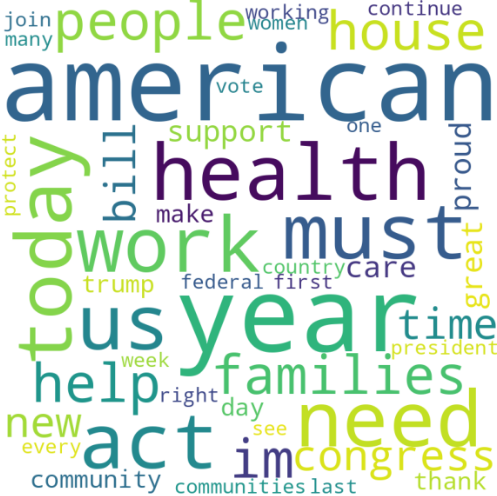
\includegraphics[width=0.7\linewidth]{images/Kapitel3/Democrat_word_cloud.png}
%  \caption{Democrat Top 50 most used words}
%  \label{fig:sub2}
	\caption{\label{fig:sub2}Democrat Top 50 most used words}{}
\end{figure}

In figure ~\ref{fig:sub1} and figure ~\ref{fig:sub2} we are able to see the top 50 most used words for the respective parties. It is interesting to note, that both parties mentions the other parties in their tweets more often than their own. Both the Republican and Democrat party used many positive words, such as people and family.

\begin{figure}
  \centering
  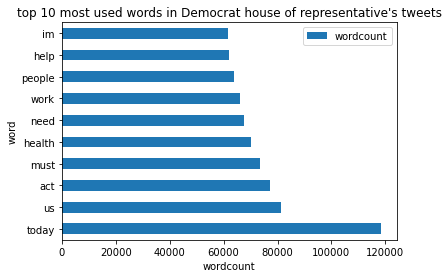
\includegraphics[width=0.8\linewidth]{images/Kapitel3/Democrat_Top_10.png}
%  \caption{Top 10 most used words by Democrats}
%  \label{fig:boat1}
	\caption{\label{fig:boat1}Top 10 most used words by Democrats}{}
\end{figure}

\begin{figure}
  \centering
  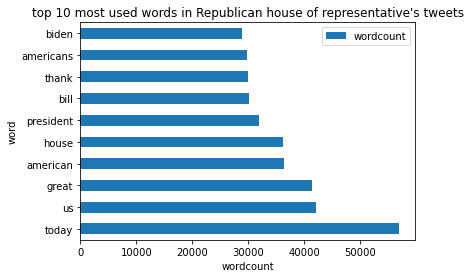
\includegraphics[width=0.8\linewidth]{images/Kapitel3/Republican_Top_10.png}
%  \caption{Top 10 most used words by Republicans}
%  \label{fig:boat2}
	\caption{\label{fig:boat2}Top 10 most used words by Republicans}{}
\end{figure}

Here in ~\ref{fig:boat1} and ~\ref{fig:boat2}, we can see it more clearly, the top 10 most used words by each parties. However in both figure, we are not able to differentiate the word us or U.S. (abbreviation for the United State), since in the preprocessing part of the pipeline, we made the words case-insensitive. These two are plotted and prepared using Pandas and \textit{Matplotlib}. 


\subsection{Sentiment Analysis}

In the project we have done sentiment analysis of the tweets using the library \textit{TextBlob}. The visualisation is made through scatter plots. The X-axis represents the polarity and the Y-Axis represents the subjectivity. The polarity explains the sentiment of the party towards general or a certain topic, whereas the subjectivity explains how subjective or objective the tweets are. Polarity of 1 expresses positiveness and -1 negativeness. Subjectivity of 1 means that the tweet was really subjective and 0 means that the tweet is really based on the truth (according to our \textit{TextBlob} library).

In ~\ref{fig:boat3}, each of the dots represent a member of the House of Representatives. From this figure, it is seen that the polarity tends to be positive. It can be concluded that from this library the sentiment towards Germany is relatively positive. However, the result is bounded by the library \textit{TextBlob} and does not represent perfectly the real sentiment that the party members carry in their tweets. More figures can be seen in the Appendix.

\begin{figure}
  \centering
  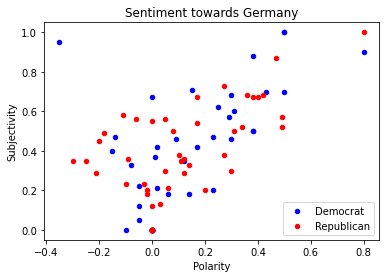
\includegraphics[width=0.7\linewidth]{images/Kapitel3/Sentiment_Germany.png}
%  \caption{Sentiment towards Germany}
%  \label{fig:boat3}
	\caption{\label{fig:boat3}Sentiment towards Germany}{}
\end{figure}
